\documentclass[12pt,a4paper]{article}
\usepackage[utf8]{inputenc}
\usepackage[italian]{babel}
\usepackage{graphicx}
\usepackage{amsmath}
\usepackage{geometry}
\usepackage{parskip}
\usepackage{svg}

\geometry{margin=1in}

\usepackage{xcolor}
\usepackage{hyperref}

\definecolor{spotifyPurple}{HTML}{B026FF}

\hypersetup{
    colorlinks=true,
    linkcolor=spotifyPurple,
    citecolor=spotifyPurple,
    urlcolor=spotifyPurple,
    linktoc=all,
    pdfborder={0 0 0}
}

\title{\textbf{Analisi delle Collaborazioni su Spotify nella Scena Musicale Ispanofona}}
\author{Francesco Giovanni Pasqual \\ Social Network Analysis [CT0540]}
\date{Anno 2025/2026}

\begin{document}

\maketitle

\section{Introduzione e Domanda di Ricerca}
Nel mercato discografico contemporaneo, le collaborazioni, o \textit{featuring}, hanno cessato di essere semplici eventi artistici sporadici per trasformarsi in pilastri strategici di posizionamento commerciale. Nella scena ispanofona, questo fenomeno è particolarmente evidente poiché ogni giorno centinaia di artisti si uniscono per mescolare le proprie \textit{fan base} e produrre canzoni uniche. Il presente lavoro indaga sulle motivazioni e pattern esistenti nella creazione di tali interconnessioni.

\textit{Quali sono i fattori che spingono gli artisti della scena ispanofona a collaborare? Sono la somiglianza di genere musicale e popolarità a dominare l'ecosistema, o esiste una spinta strategica verso la connessione di scene geograficamente e stilisticamente distanti?}

\newpage

\section{Riferimenti Scientifici}
Per supportare l'analisi sono stati selezionati sei contributi che affrontano la teoria delle reti applicata all'industria creativa:

\begin{enumerate}
    \item \textbf{Small-World Properties in Spotify} (R. A. Magalhães Bush, 2025): conferma la natura \textit{small-world} delle reti musicali, evidenziando come diametri ridotti e hub centrali facilitino una rapida diffusione delle tendenze. \href{https://papers.cool/arxiv/2503.09526}{Web}
    
    \item \textbf{Music-Genre Dependence of Graph Metrics} (G. Clerici e M. Tiraboschi, 2023): introduce un indice di reciprocità per distinguere le collaborazioni reali dalle semplici citazioni, dimostrando che l'alta centralità dell'\textbf{Hip-hop} è il risultato di una cultura collaborativa strutturata e reciproca. \href{https://air.unimi.it/handle/2434/997649}{Web}
    
    \item \textbf{Collaboration Patterns in Genre Networks} (G. P. Oliveira e M. M. Moro, 2022): descrive le collaborazioni tra generi diversi come strumenti fondamentali per superare i confini di nicchia e creare ponti tra mercati stilistici differenti. \href{https://www.researchgate.net/publication/372946800_Exceptional_Collaboration_Patterns_in_Music_Genre_Networks}{Web}
    
    \item \textbf{Impact of Homophily on Song Popularity} (N. Reisz, V. D. P. Servedio e S. Thurner, 2024): analizza l'omofilia come driver principale di connessione, dimostrando che la somiglianza tra artisti influenzi direttamente la probabilità di successo dei brani. \href{https://pmc.ncbi.nlm.nih.gov/articles/PMC11026404/}{Web}
    
    \item \textbf{Spotify Artist Collaboration Graph} (T. South, 2018): propone un framework per l'analisi strutturale dei \textit{grafi} di collaborazione estratti direttamente tramite le \textit{API} della piattaforma \textbf{Spotify}. \href{https://vrs.amsi.org.au/wp-content/uploads/sites/84/2018/04/tobin_south_vrs-report.pdf}{Web}
\end{enumerate}

\newpage

\section{Metodologia di Raccolta Dati e Costruzione della Rete}
I dati sono stati estratti tramite le \textit{API} ufficiali di \textit{Spotify for Developers} utilizzando la libreria Python \textit{Spotipy}. La strategia di campionamento adottata è lo \textit{snowball sampling}.
Sono stati selezionati 50 artisti di riferimento (\textit{seeds}) rappresentativi dei leader della scena ispanofona in diversi stati: tra questi figurano, ad esempio, \textbf{Bad Bunny} (Porto Rico), \textbf{Peso Pluma} (Messico) e \textbf{Saramalacara} (Argentina). 

La ricerca è stata limitata a un singolo livello di profondità, ovvero per ogni seed sono stati analizzati gli ultimi 50 brani (tra album e singoli) per identificarne i collaboratori. La rete è stata costruita collegando l'artista titolare del brano (\textit{source}) ai suoi collaboratori (\textit{target}). Nel caso di brani con più \textit{featuring}, sono stati creati collegamenti anche tra i collaboratori stessi, in modo da mappare l'intero gruppo di artisti che hanno lavorato insieme. Per un maggiore approfondimento visionare il bias \hyperref[s:primobias]{1}.

Il software \textit{Gephi} è stato utilizzato per la visualizzazione e il calcolo delle metriche sul \textit{grafo}; lo stesso ha inoltre permesso di individuare le comunità all'interno della rete e colorarle attraverso una palette cromatica, applicata coerentemente a tutte le figure presenti nel progetto.

\newpage

\section{Analisi dei Risultati e Visualizzazioni}

\subsection{Indicatori Statistici e Risultati Quantitativi}

La rete analizzata presenta caratteristiche strutturali ben definite, riassunte dalle seguenti metriche:
\begin{itemize}
    \item \textbf{Densità:} $0.005$. Il valore estremamente basso indica una rete \textit{sparsa}, coerente con la vastità del panorama musicale dove non tutti possono collaborare con tutti.
    \item \textbf{Average Path Length:} $3.596$. Nonostante la bassa densità, ogni artista è mediamente separato da un altro da meno di 4 \textit{passaggi}, confermando le proprietà \textit{small-world} citate in letteratura.
    \item \textbf{Diametro:} $8$. La distanza massima tra due nodi è contenuta, suggerendo una rete coesa.
    \item \textbf{Modularità ($0.524$):} Questo indice misura il grado di divisione della rete in gruppi o comunità. Poiché in letteratura valori superiori a 0.4 indicano una struttura comunitaria marcata, il risultato ottenuto conferma una forte segmentazione della scena ispanofona. Gli artisti tendono a gravitare all'interno di \textit{cluster} densamente connessi, suggerendo che le collaborazioni avvengono prevalentemente all'interno di cerchie specifiche piuttosto che in modo uniforme sull'intera rete.
\end{itemize}

\newpage

\subsection{Interpretazione Visuale della Rete}

Dall'osservazione della Figura \ref{fig:rete} emerge chiaramente che la scena musicale ispanofona non è un gruppo unico e uniforme. Al contrario, è formata da diversi sottogruppi (\textit{cluster}), spesso molto collegati tra di loro.

Alcune di queste comunità sono molto chiuse e compatte, come nel caso dei \textbf{Corridos} messicani o della \textbf{Trap} argentina, dove gli artisti collaborano quasi esclusivamente a vicenda. Altri artisti, invece, si trovano in una posizione intermedia e fungono da \textit{ponti} tra i vari gruppi, permettendo a generi diversi di mescolarsi.

\begin{figure}[h!]
    \centering
    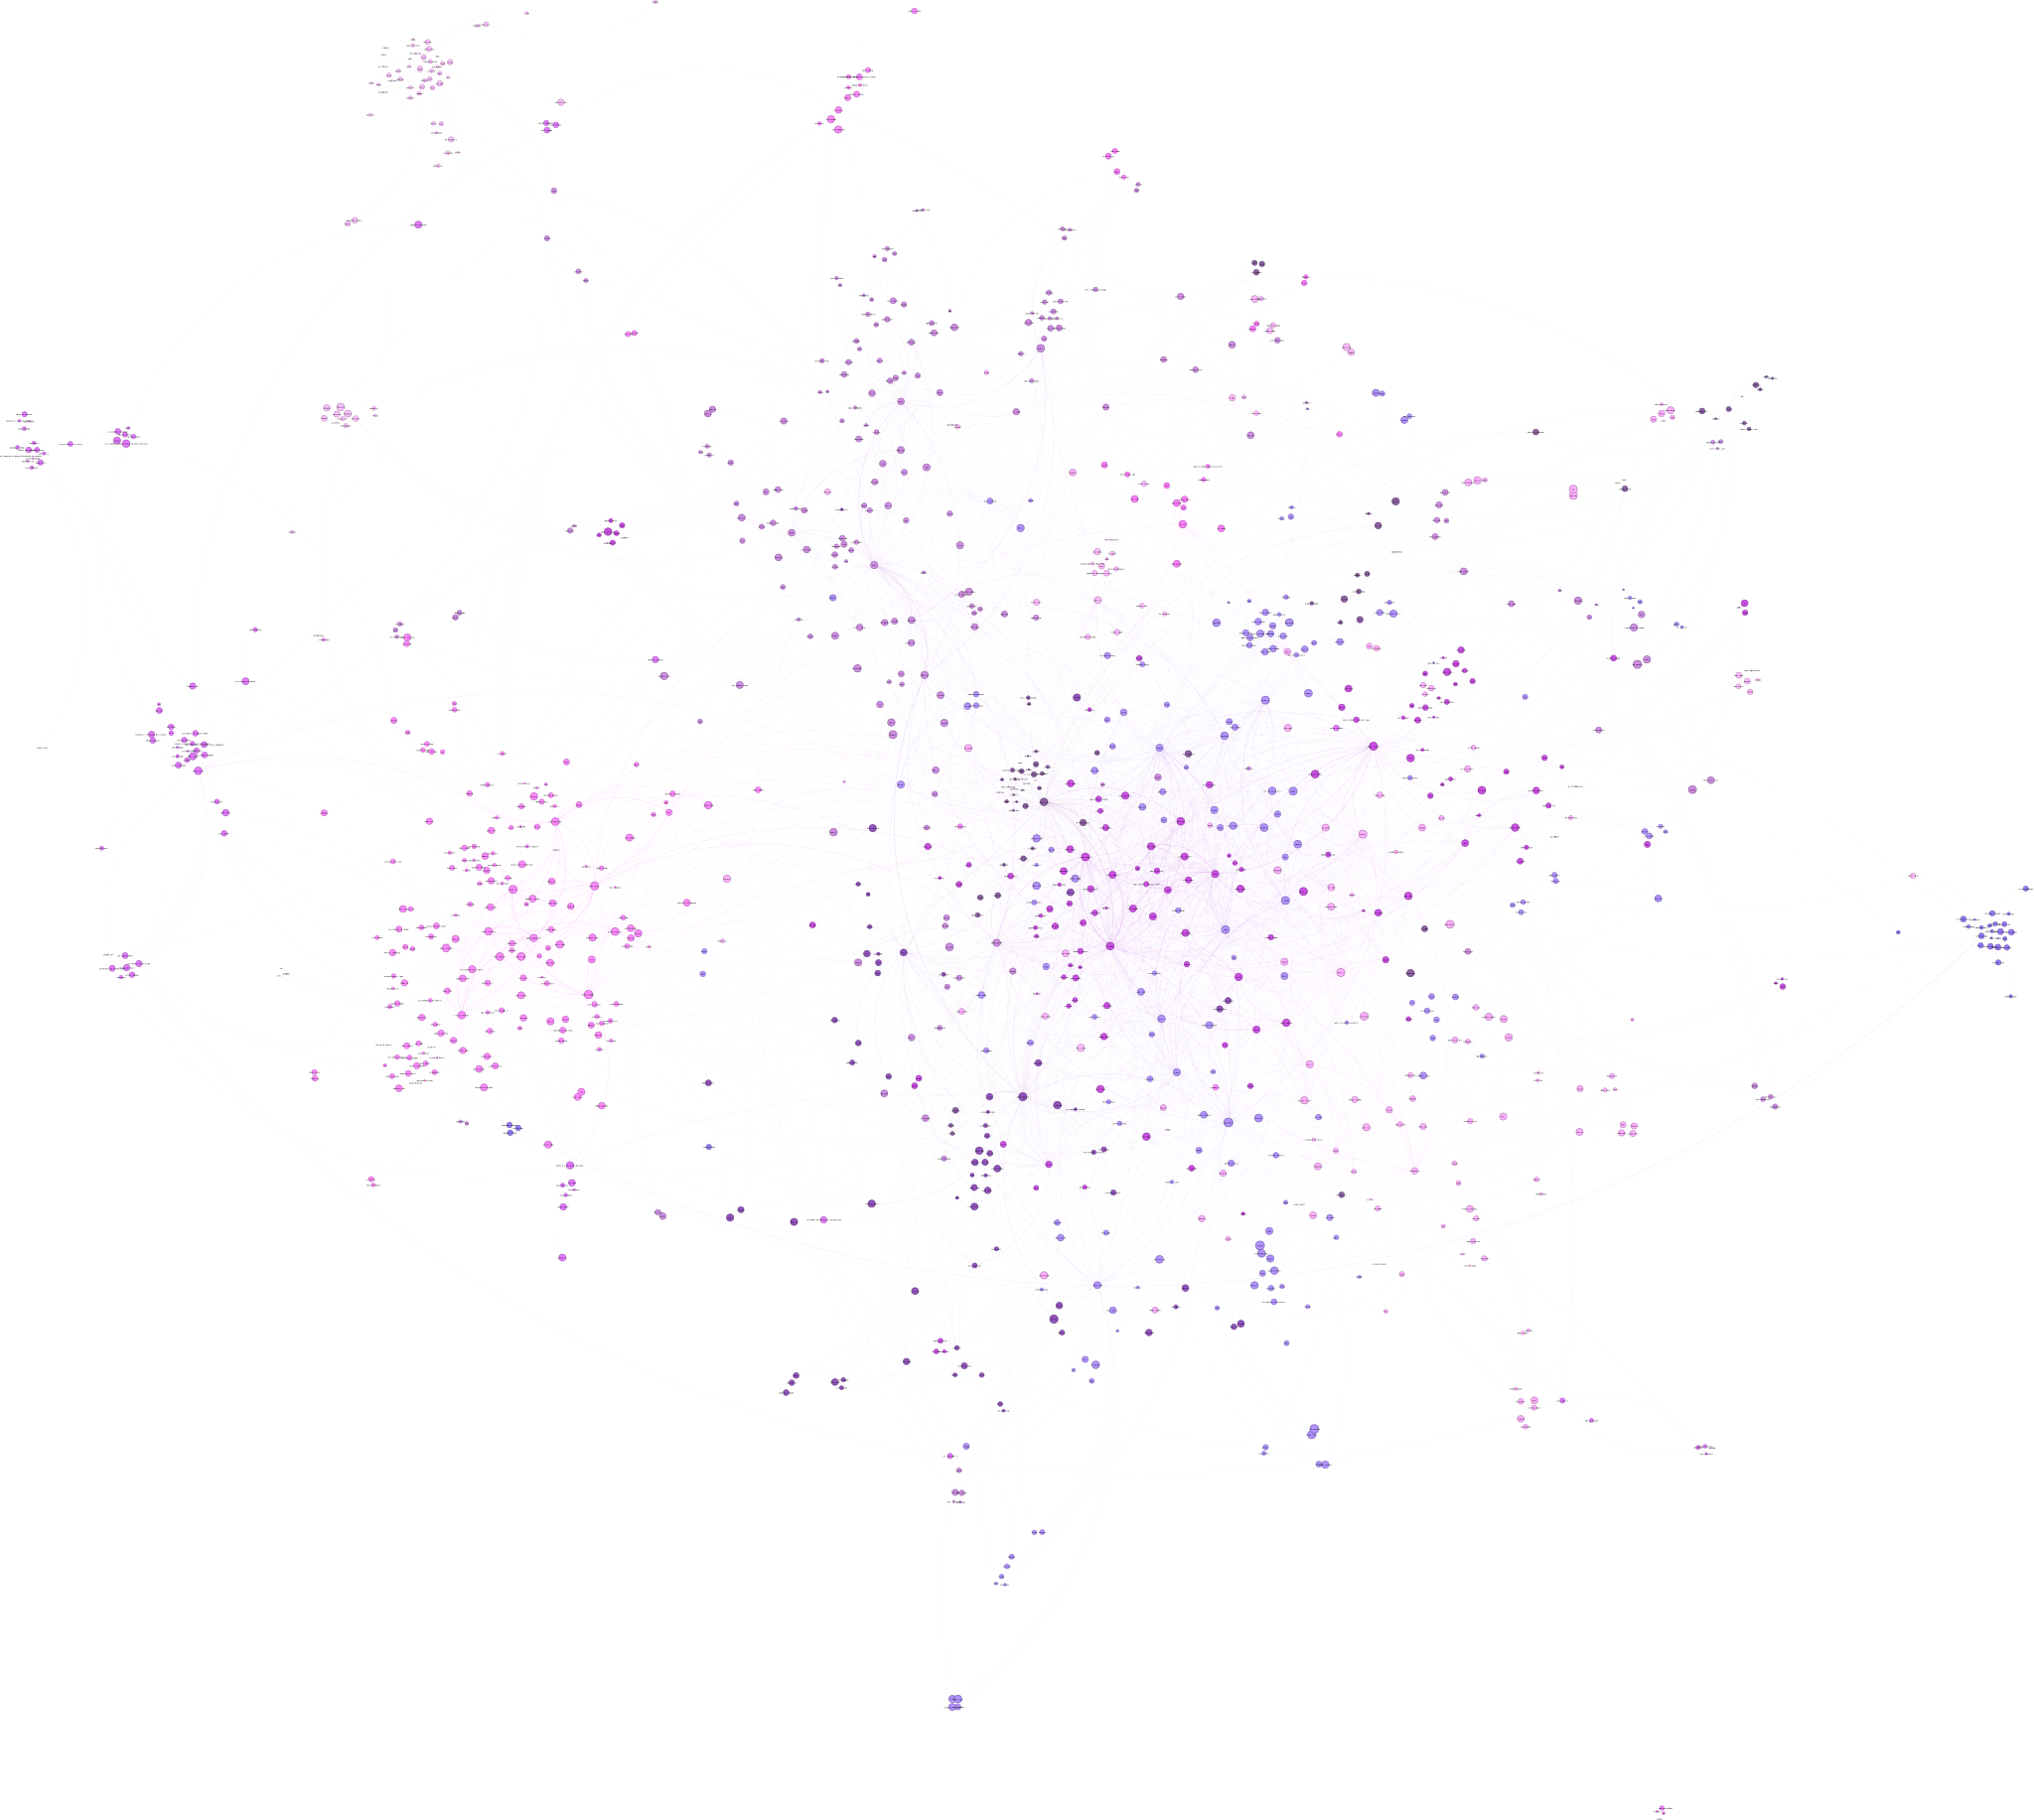
\includegraphics[width=0.7\linewidth]{rete.pdf}
    \caption{\textit{Grafo} delle collaborazioni ispanofone. La colorazione dei nodi riflette le comunità individuate dall'algoritmo di \textit{Louvain} all'interno di \textit{Gephi}, mentre la dimensione dei nodi e quella del testo sono proporzionali al grado di popolarità dell'artista.}
    \label{fig:rete}
\end{figure}

\newpage

\subsection{Omofilia di Genere}
Per comprendere meglio i criteri che guidano le collaborazioni, l'analisi si è focalizzata sul fenomeno dell'\textit{omofilia}, ovvero la tendenza degli artisti a connettersi con colleghi che condividono lo stesso stile musicale. La heatmap in Figura \ref{fig:heatmap} permette di visualizzare la distribuzione dei generi musicali all'interno delle diverse comunità individuate da \textit{Gephi}.

L'osservazione dei dati conferma l'ipotesi iniziale, in cui le comunità non sono gruppi casuali, ma sono fortemente caratterizzate da uno o due generi dominanti. Questo suggerisce che, nonostante la globalizzazione del mercato, il genere musicale rimane il principale motore di aggregazione nella scena ispanofona.

\begin{figure}[h!]
    \centering
    \includegraphics[width=0.8\textwidth]{heatmap.png}
    \caption{Heatmap della distribuzione dei generi per comunità. Le righe rappresentano le comunità, denominate in base all'artista più popolare che rappresenta il genere dominante del gruppo, mentre le colonne indicano i generi musicali. Si noti che il totale per riga può superare il 100\% poiché per ogni artista sono stati considerati i due generi principali.}
    \label{fig:heatmap}
\end{figure}

\newpage

\subsection{Omofilia di Status}
Un altro aspetto fondamentale dello studio riguarda la relazione tra la fama dell'artista che \textit{ospita} (\textit{Source}) e quella dell'artista che \textit{partecipa} al brano (\textit{Target}). Lo scatterplot in Figura \ref{fig:scatter} mette a confronto queste due variabili per verificare se esista una tendenza a collaborare solo tra pari livello.

Sebbene si noti una forte concentrazione di punti lungo la diagonale, specialmente nella parte in alto a destra, segno di una chiara \textit{omofilia di status} dove artisti con popolarità simile tendono a lavorare insieme, lo scatterplot rivela anche numerose eccezioni. Molti punti si collocano infatti lontani dalla diagonale, indicando collaborazioni tra artisti con livelli di popolarità molto distanti. Questo dato suggerisce che, anche se la fama sia un fattore influente, essa non è un vincolo assoluto dal momento che la scena ispanofona è caratterizzata da una dinamicità che permette anche ad artisti emergenti di entrare in contatto con i grandi nomi del settore.

\begin{figure}[h!]
    \centering
    \includegraphics[width=0.8\textwidth]{scatterplot.png}
    \caption{Scatterplot della popolarità. Artista \textit{Source} a confronto con Artista \textit{Target}. La disposizione dei punti lungo la diagonale indica una relazione diretta tra la popolarità dei due collaboratori. I punti distanti dalla diagonale rappresentano invece collaborazioni tra artisti con livelli di fama differenti.}
    \label{fig:scatter}
\end{figure}

\newpage

\subsection{Analisi Geografica}

L'analisi della distribuzione geografica dalla Figura \ref{fig:nazioni} evidenzia una forte \textit{omofilia nazionale}, con \textit{self-loops} marcati dettati dal radicamento territoriale dei generi e specialmente i loro sottogeneri. Un esempio molto evidente è quello dei \textbf{Corridos} messicani, poiché la loro specifica connotazione culturale spinge gli artisti a collaborare prevalentemente tra di loro, saturando la rete locale. In questo scenario, l'\textit{omofilia} di genere si traduce inevitabilmente in \textit{omofilia geografica}. Al contrario, le collaborazioni transnazionali emergono come scelte strategiche in contesti più \textit{mainstream} per l'ibridazione dei mercati e delle \textit{fanbase} differenti. Infine, la rilevante centralità degli Stati Uniti richiede una lettura critica, legata alle ambiguità metodologiche chiarite nel bias \hyperref[s:quartobias]{4}.

\begin{figure}[h!]
    \centering
    \includegraphics[width=0.7\textwidth]{nazioni.pdf}
    \caption{\textit{Grafo} delle collaborazioni aggregate per nazione. La colorazione dei nodi è casuale e lo spessore dei collegamenti indica il \textit{peso} della relazione tra una nazione e un'altra. La dimensione dei nodi è variabile in base al grado del nodo e il testo è fisso per motivi di visibilità.}
    \label{fig:nazioni}
\end{figure}

\subsection{Analisi delle Metriche per i Singoli Artisti}

L'analisi statistica della rete permette di andare oltre l'aspetto puramente visivo, quantificando l'influenza delle star attraverso diversi strumenti di centralità, che mirano a studiare i veri motori strutturali del network. 

La \textit{Betweenness Centrality} vede primeggiare \textbf{Duki} ($0.135$), seguito da \textbf{Arcángel} ($0.109$) e \textbf{Ñengo Flow} ($0.093$). L'alto valore di \textbf{Duki} ne conferma il ruolo di mediatore culturale tra la \textbf{Trap} argentina e il \textbf{Reggaeton} portoricano. Anche artisti come \textbf{Becky G} ($0.091$) e \textbf{Luis R Conriquez} ($0.083$) emergono come connettori strategici tra generi distanti.

Per prestigio e integrazione nel core del network, la \textit{Eigenvector Centrality} e il \textit{Weighted Degree} vedono il dominio di \textbf{Arcángel} ($1.000$ e $192$ collaborazioni), seguito da \textbf{Yandel} ($0.933$) ed \textbf{Eladio Carrión} ($0.834$), che rappresentano l'élite consolidata del genere \textbf{Trap} latinoamericana.

Un'osservazione fondamentale emerge infine dall'analisi della \textit{Closeness Centrality}, ovvero la capacità di un nodo di raggiungere rapidamente tutti gli altri. Questo numero è guidato ancora da \textbf{Arcángel} ($0,431$), seguito da \textbf{Myke Towers} ($0,425$) ed \textbf{Eladio Carrión} ($0,420$). All'interno di questo parametro finalmente, e per la prima volta, troviamo \textbf{Bad Bunny} e \textbf{Peso Pluma} che, pur essendo due degli artisti con le popolarità più alte in assoluto, \textbf{Bad Bunny} ($98/100$) e \textbf{Peso Pluma} ($89/100$), non figurano tra i primi per nessuna delle altre metriche di centralità. 

Questo suggerisce che la loro influenza è più legata alla qualità della loro musica, in molti casi come singoli, e alla loro vicinanza con altri nodi ben connessi della rete, più che a un ruolo di mediatore tra nicchie isolate, oppure di numerosi e frequenti \textit{featuring}. Diventa quindi evidente che la fama commerciale e la funzione strutturale nel network sono dinamiche distinte che rispondono a logiche diverse del mercato musicale.

\newpage

\section{Limiti e Bias dell'Analisi}
Molto spesso analisi di rete basati su dati estratti via \textit{API} comportano dei bias intrinseci che devono essere riconosciuti per una corretta interpretazione dei risultati:

\begin{enumerate}
    \item \textbf{Selezione dei \textit{Seed} e Metodologia di Raccolta:} 
        \begin{itemize}
            \item \label{s:primobias} \textbf{Distribuzione e scelta dei Seed:} I 50 artisti iniziali sono stati scelti manualmente sulla base della conoscenza diretta della scena ispanofona maturata dall'autore durante la sua permanenza in Messico. Sebbene questo approccio garantisca l'inclusione di figure cardine, introduce un bias soggettivo verso i mercati più noti, lasciando in secondo piano contesti pur rilevanti (es. Colombia, Cile o Venezuela). Sono state evitate classifiche esterne, spesso poco fedeli alle reali dinamiche di ascolto, per preservare l'integrità dei dati ed evitare \textit{rumore} analitico. Ci si è quindi concentrati sui mercati dominanti e verificabili per esperienza diretta.

            I 50 \textit{seed} sono così distribuiti: \textbf{Messico} (16), \textbf{Puerto Rico} (13), \textbf{Argentina} (9), \textbf{USA} (5), \textbf{Spagna} (3), \textbf{Colombia} (2), \textbf{Cile} (1) e \textbf{Panama} (1).
        
            \item \textbf{Gestione del Volume Dati e Limitazioni \textit{API}:} Il campionamento è stato limitato a 50 seed e a un solo livello di profondità per ragioni tecniche. Un numero superiore di nodi avrebbe reso il dataset eccessivamente vasto e difficile da elaborare; inoltre, l'estrazione massiva di dati espone al rischio di blocchi, \textit{rate limiting}, da parte delle \textit{API} di Spotify.
        \end{itemize}
    
    \item \textbf{Orizzonte Temporale:} L'analisi considera solo gli ultimi 50 brani per artista. Questa scelta è motivata dalla volontà di fotografare lo stato attuale dell'industria musicale, evitando che collaborazioni datate, non più rappresentative della posizione attuale dell'artista nel mercato, influenzino la struttura della rete contemporanea.

    \item \textbf{Mapping dei Generi:} Data la vastità dei tag di \textbf{Spotify}, i generi sono stati uniti in categorie più estese. Questa semplificazione, necessaria per la leggibilità della heatmap, può nascondere sfumature artistiche e sottogeneri importanti.
    
    \item \label{s:quartobias} \textbf{Dati Geografici e Ambiguità della \textit{Nazionalità}:} Il concetto di \textit{nazionalità} nel dataset è spesso ambiguo. Molti artisti nati in America Latina risiedono o producono negli USA, contribuendo a gonfiare i dati degli Stati Uniti pur mantenendo un background culturale ispanico. Inoltre, circa poco meno della metà del dataset manca di informazioni geografiche precise, rendendo il grafo delle proiezioni nazionali meno solido statisticamente.
\end{enumerate}

\newpage

\section{Conclusioni}

Sintetizzando, l'analisi del network ispanofono delinea un ecosistema dinamico dove l'\textit{omofilia di status} non è il vincolo principale. Le collaborazioni tra artisti con popolarità differenti sono frequenti, guidate primariamente da affinità musicali e culturali. Il \textit{featuring} si conferma non solo uno strumento di espansione delle \textit{fanbase}, ma un atto di allineamento stilistico necessario alla coerenza artistica dei partecipanti.

L'integrazione strutturale è l'elemento più rilevante della ricerca. L'\textit{Average Path Length} di soli all'incirca tre \textit{passi} e mezzo evidenzia proprietà \textit{small-world} marcate. Tale vicinanza suggerisce un potenziale di inserimento rapido per gli artisti emergenti, per i quali un singolo legame strategico all'interno del proprio genere può fungere da catalizzatore per una scalata accelerata verso il nucleo della rete.

Infine, sempre facendo riferimento alla ridotta distanza media, essa garantisce una diffusione fulminea di tendenze e innovazioni, nonostante la bassa densità complessiva del sistema. Quello che appare come un insieme di nicchie isolate si rivela, alla prova dei dati, un organismo interconnesso dove la prossimità strutturale prevale nettamente sulla distanza geografica o commerciale.

\newpage

\section{Bibliografia}

\begin{itemize}
    \item Magalhães Bush, R. A. (2025). \textit{Analysis of a Spotify Collaboration Network for Small-World Properties}. Disponibile all'indirizzo: \href{https://papers.cool/arxiv/2503.09526}{Web}
    
    \item Clerici, G., \& Tiraboschi, M. (2023). \textit{Citation is not Collaboration: Music-Genre Dependence of Graph-Related Metrics in a Music Credits Network}. Disponibile all'indirizzo: \href{https://air.unimi.it/handle/2434/997649}{Web}
    
    \item Oliveira, G. P., \& Moro, M. M. (2022). \textit{Exceptional Collaboration Patterns in Music Genre Networks}. Disponibile all'indirizzo: \href{https://www.researchgate.net/publication/372946800_Exceptional_Collaboration_Patterns_in_Music_Genre_Networks}{Web}
    
    \item Reisz, N., Servedio, V. D. P., \& Thurner, S. (2024). \textit{Quantifying the impact of homophily and influencer networks on song popularity prediction}. Disponibile all'indirizzo: \href{https://pmc.ncbi.nlm.nih.gov/articles/PMC11026404/}{Web}
    
    \item South, T. (2018). \textit{Network Analysis of the Spotify Artist Collaboration Graph}. Disponibile all'indirizzo: \href{https://vrs.amsi.org.au/wp-content/uploads/sites/84/2018/04/tobin_south_vrs-report.pdf}{Web}
\end{itemize}

\vfill
\begin{center}
\tiny Documento redatto in \LaTeX.
\end{center}

\end{document}